\chapter{Hamiltonian Equation of Motion}
 Hamiltonian method providing a framework for theoretical basis for further developments like Hamiltonian Jacobi theory, perturbation approaches and chaos. Outside classical mechanics Hamiltonian formulation provides much of the language with which present-day statistical mechanics and quantum mechanics is constructed. Throughout the chapter we are assuming mechanical systems are holonomic and the forces are monogenic.
 \begin{itemize}
 	\item In Hamiltonian formulation there can be no constraint equation among the coordinates.
 	\item If $n$ coordinates are not independent, a reduced set of $m$ coordinates, with $m<n$, must be used for the formulation of the problem
 \end{itemize}
\section{Hamiltonian Formulation}
\begin{itemize}
	\item Describe the motion in terms of first order equations of motion
	\item Number of initial conditions determining the motion are stil be $2n$
	\item $2n$ independent first order equations expressed in terms of $2n$ independent variables
	\item $2n$ equations of motion describe behavior of the system point in a phase space
	\item Out of $2n$ independent quantities half of them are $n$ generalized coordinates and other half set to be the generalized or conjugate momenta $p_i$
	\begin{equation}
	  p_i=\frac{\partial L(q_j,\dot{q}_j, t)}{\partial \dot{q}_j}
	\end{equation}
	where $j$ index shows the set of $q$'s and $\dot{q}$'s
	\item The quantities $(p,q)$ are known as the canonical variables
\end{itemize}
\section{Legendre Transformation}
Consider a function of only two variables $f(x,y)$ so that a differential of $f$ has the form
$$df=udx+vdy$$
where
$$u=\frac{\partial f}{dx},\quad v=\frac{\partial f}{dy}$$
To change the basis of description from $x,y$ to a new distinct set of variables $u,y$ so that differential quantities are expressed in terms of $du$ and $dy$
\begin{align*}
\intertext{Let $g$ be a function $u$ and $y$ defined by the equation}
g&=f-ux
\intertext{A differential of $g$ is then given as}
dg&=df-udx-xdu
\intertext{or}
dg&=vdy-xdu
\intertext{and we get}
x=\frac{-\partial g}{\partial u},&\quad v=\frac{\partial g}{\partial y}
\end{align*}
\section{Hamilton Equation of Motion}
Mathematically the transition from Lagrangian to Hamiltonian formulation corresponds to changing the variables in our mechanical functions from $(q, \dot{q}_j,t)$ to $(q,p,t)$ when $p$ is related to $q$ and $\dot{q}$ by
$$p_i=\frac{\partial L(q_j,\dot{q}_j,t)}{\partial \dot{q}_i}$$
The proceedure for switching variables in this manner is provided by the 'Legendre  transformation'.
\begin{align}
\text{Consider Lagrangian }&\ L(q,\dot{q},t)\ \text{ then}\notag\\
dL=\frac{\partial L}{\partial q_i}dq_i&+\frac{\partial L}{\partial \dot{q}_1}+\frac{\partial L}{\partial t}dt\\
\text{The canonical }&\text{momentum  was defined as }p_i=\frac{\partial L}{\partial \dot{q}_i}\notag\\
\text{Substituting it in }&\text{Lagrange equation we obtain}
\dot{p}_i=\frac{\partial L}{\partial {q}_i}\notag\\
\therefore dL&=\dot{p}_idq_i+p_id\dot{q}_i+\frac{\partial L}{\partial t}dt
\intertext{The Hamiltonian $H(q,p,t)$ is generated by the Legendre transformation}
H(q,p,t)&=\dot{q}_ip_i-L(q,\dot{q},t)
\intertext{and has the differential}
dH&=\dot{q}_1dp_i-\dot{p}_1dq_1-\frac{\partial L}{\partial t}dt
\intertext{Where the term $p_id\dot{q}_i$ removed by Legendre transformation since $dH$ can also written as }
dH&=\frac{\partial H}{\partial q_i}dq_1+\frac{\partial H}{\partial p_i}dp_i+\frac{\partial H}{dt}dt
\intertext{We obtain $2n+1$ relations}
&\left.\begin{array}{rl}\dot{q}_{i} & =\frac{\partial H}{\partial p_{i}} \label{HM-07}\\\\ -\dot{p}_{i} & =\frac{\partial H}{\partial q_{i}}\end{array}\right\}\\\notag\\
&-\frac{\partial L}{\partial t}=\frac{\partial H}{\partial t}\notag
\end{align}
Equation $\ref{HM-07}$ are known as the canonical equations of Hamiltonian
\section{Steps to construct Hamiltonian}
Hamiltonian for each problem must be constructed via the Lagrangian formulation.
\begin{enumerate}
	\item With chosen set of generalized coordinates, $q_i$ the Lagrangian $L(\dot{q},\dot{q}_i,t)$=T-V is constructed
	\item The conjugate momenta are defined as function of $q_i,\dot{q}_i$ and $t$ by equation
	$$p_i=\frac{\partial L}{\partial \dot{q}_i}$$
	\item Legendre transformation used to form the Hamiltonian. At this stage we have some mixed functions of $q_i,\dot{q}_i,p_i$ and $t$
	\item $p_i=\frac{\partial L}{\partial \dot{q}_i}$ then converted to obtain $\dot{q}_i$ as functions of $(q,p,t)\ (ie\quad \dot{q}_i=\frac{\partial H}{\partial p_i})$
	\item The result of the previous steps are then applied to eliminate $\dot{q}_i$ from $H$ so to express it solely as a function of $(q,p,t)$
\end{enumerate}
\begin{note}
	In many problems Lagrangian is the sum of functions each homogeneous in the generalized velocities of degree $0,1$ and $2$ respectively in that are
	$$ H=\dot{q}_1p_i-L=\dot{q}_ip-[L_0(q,t)+L_i(q,t)\dot{q}_k+L_1(q_i,t)\dot{q}_k\dot{q}_m]$$
	If equations defining generalized coordinates don't depend on time then $L_2 \dot{q}_k\dot{q}_m=T(K.E)$\\
	If forces are derivable from a consevative potential $V$ (ie work is independent of path), then $L_0=-V$
	When both there conditions are satisfied the Hamiltonian is automatically the total energy
	$$H=T+V=
	E$$
\end{note}
\begin{exercise}
	A particle of inass $m$ moves inside a bowl under gravity. If the surface of the bowl is given by the equation $z=\frac{1}{2} a\left(x^{2}+y^{2}\right)$, where $a$ is a constant.\\
	(A) Write down Lagrangian of the system in cylindrical co-ordinate.\\
	(a) Identified the cyclic coordinate and law of conservation of momentum.\\
	(b) Write down hamiltonion of the system in cylindrical coordinate system.
\end{exercise}
	\begin{answer}
	\begin{align*}
	\text{(A) }T&=\frac{1}{2} m\left(\dot{r}^{2}+r^{2} \dot{\theta}^{2}+\dot{z}^{2}\right)=\frac{m}{2}\left(\dot{r}^{2}+r^{2} \dot{\theta}^{2}+a^{2} r^{2} \dot{r}^{2}\right) \quad \because z=\frac{1}{2} a r^{2} \Rightarrow \quad \dot{z}=a r \dot{r}\\
	V&=m g z=\frac{1}{2} m g a r^{2} \\
	L&=\frac{m}{2}\left[\dot{r}^{2}\left(1+a^{2} r^{2}\right)+r^{2} \dot{\theta}^{2}-a g r^{2}\right]
	\intertext{	(a) $\theta$ is cyclic coordinate}
	\because \frac{\partial L}{\partial \theta}&=0, \Rightarrow \dot{p}_{\theta}=0 \Rightarrow P_{\theta}=\text{ constant}
	\intertext{(b) Hamiltonian}
	H&=\frac{p_{r}^{2}}{2 m\left(1+a^{2} r^{2}\right)}+\frac{p_{\theta}^{2}}{2 m r^{2}}+\frac{1}{2} m a g r^{2} \quad \\&\because \frac{\partial L}{\partial \dot{r}}=p_{r}=m\left(1+a^{2} r^{2}\right) \dot{r}\text{ and }\frac{\partial L}{\partial \dot{\theta}}=p_{\theta}=m r^{2} \dot{\theta}
	\end{align*}
\end{answer}
\begin{exercise}
	A particle of mass $m$ is attached to fixed point $O$ by a weightless inextensible string of length $a$. It is rotating under the gravity as shown in the figure.\\
	(a) Write down The Lagrangian of the system in spherical co-ordinate.\\
	(b) write down Hamiltonian of the system.
	\begin{figure}[H]
		\centering
		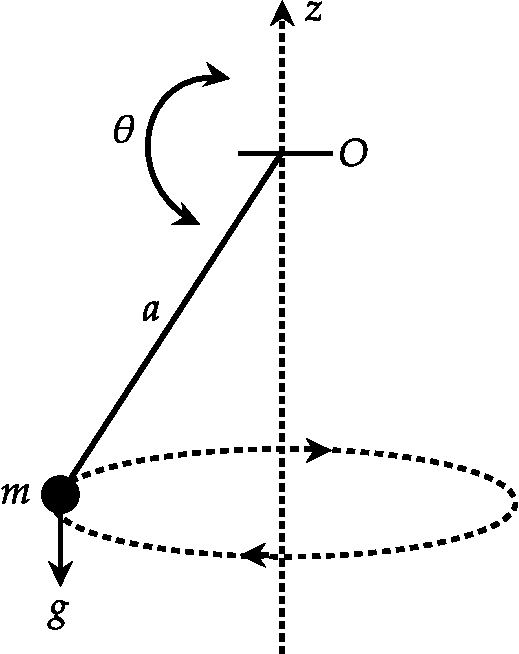
\includegraphics[height=4.5cm,width=3.5cm]{Assignment-HE-02}
	\end{figure}
\end{exercise}
	\begin{answer}
	\begin{align*}
	L&=\frac{1}{2} m\left(\dot{x}^{2}+\dot{y}^{2}+\dot{z}^{2}\right)-[m g(-z)]\\
	L&=\frac{1}{2} m\left(a^{2} \dot{\theta}^{2}+a^{2} \sin ^{2} \theta \dot{\phi}^{2}\right)+m g a \cos (\pi-\theta)\\
	L&=\frac{1}{2} m\left(a^{2} \dot{\theta}^{2}+a^{2} \sin ^{2} \theta \dot{\phi}^{2}\right)-m g a \cos (\theta)\\
	H&=\sum \dot{q}_{1} p_{1}-L\\
	H&=\frac{p_{\theta}^{2}}{2 m a^{2}}+\frac{p_{\phi}^{2}}{2 m a^{2} \sin ^{2} \theta}+m a g \cos \theta \because \frac{\partial L}{\partial \dot{\theta}}=p_{\theta}=m a^{2} \dot{\theta}\text{ and } \frac{\partial L}{\partial \dot{\phi}}=p_{\phi}=m a^{2} \sin ^{2} \theta \dot{\phi}
	\end{align*}
\end{answer}
\begin{exercise}
	Particle of mass $m$ slides under the gravity without friction along the parabotic path
	$y=a x^{2}$ axis shown in the figure. Here $a$ is a constant\\
	(a) Write down Lagrangian of the system .\\
	(b) Write down Lagranges equation of motion.\\
	(c) write down Hamiltonian of the system.
	\begin{figure}[H]
		\centering
		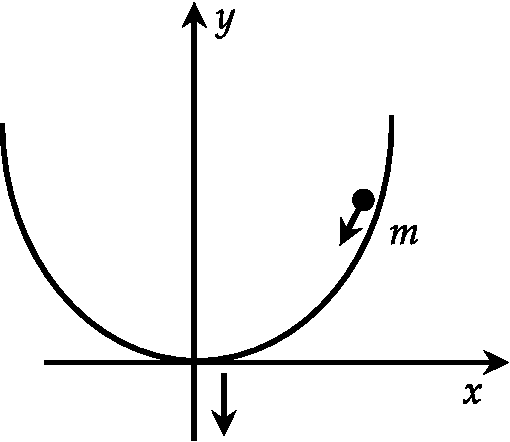
\includegraphics[height=3.5cm,width=4cm]{Assignment-HE-03}
	\end{figure}
\end{exercise}
	\begin{answer}
	\begin{align*}
	y&=a x^{2}\\
	\text{(a) }\dot{y}&=2 a x \dot{x}\\
	L&=\frac{m}{2}\left(\dot{x}^{2}+\dot{y}^{2}\right)-m g y=\frac{m}{2}\left(\dot{x}^{2}+4 a^{2} x^{2} \dot{x}^{2}\right)-m g a x^{2}\\
	L&=\frac{m}{2}\left(1+4 a^{2} x^{2}\right) \dot{x}^{2}-m g a x^{2}\\
	\text{	(b) }&\frac{d}{d t}\left(\frac{\partial L}{\partial \dot{x}}\right)-\frac{\partial L}{\partial x}=0\\
	\frac{d}{d t}&\left[m\left(1+4 a^{2} x^{2}\right) \dot{x}\right]-\left[4 m a^{2} \dot{x}^{2} x-2 \mathrm{~m} g\right.\text{ a }\left.x\right]=0\\
	m \ddot{x}&+4 m a^{2} \ddot{x} x^{2}+8 m a^{2} \dot{x} x \dot{x}-4 m a^{2} \dot{x}^{2} x+2 m g a x=0\\
	m \ddot{x}&+4 m a^{2} x^{2} \ddot{x}+4 m a^{2} x \dot{x}^{2}+2 m g a x=0\\
	\text{(c) }H&=\sum \dot{x} p_{x}-L\\
	H&=\frac{p_{x}^{2}}{2 m\left(1+4 a^{2} x^{2}\right)}+m g a x^{2} \quad \because \frac{\partial L}{\partial \dot{x}}=p_{x}=m\left(1+4 a^{2} x^{2}\right) \dot{x}
	\end{align*}
\end{answer}
\begin{exercise}
	The Lagrangian of a particle of mass $m$ moving in one dimension is $L=\exp (\alpha t)\left[\frac{m \dot{x}^{2}}{2}-\frac{k x^{2}}{2}\right]$, where $\alpha$ and $k$ are positive constants.\\
	(a) Find the Lagranges equation of motion of the particle.\\
	(b) Write down Hamiltonian of the system.
\end{exercise}
	\begin{answer}
	\begin{align*}
	L&=e^{\alpha t}\left(\frac{m \dot{x}^{2}}{2}-\frac{k x^{2}}{2}\right)\\
	\text{(a) }\frac{d}{d t}\left(e^{\alpha t} m \dot{x}\right)-e^{\alpha t} k x&=0 \Rightarrow e^{\alpha t} m \ddot{x}+m \dot{x} e^{\alpha t} \cdot \alpha-e^{\alpha t} k x=0 \Rightarrow e^{\alpha t}[m \ddot{x}+\alpha m \dot{x}-k x]=0\\
	\text{(b) }H&=e^{-\alpha t} \frac{p_{x}^{2}}{2 m}+e^{\alpha t} \frac{k x^{2}}{2}
	\because \frac{\partial L}{\partial \dot{x}}=p_{x}=e^{\alpha t} m \dot{x}
	\end{align*}
\end{answer}
\section{Cyclic Coordinate and Conservation Theorem}
If $q_j$ a cyclic coordinate then, its conjugate momentum $p_j$ is constant.\\
From Lagrangian and Hamiltonian equations of motions:
$$\dot{p}_{j}=\frac{\partial L}{\partial q_{j}}=-\frac{\partial H}{\partial q j}$$
$\therefore$ coordinate that is cyclic will thus also be absent from the Hamiltonian. Conversely if a generalized coordinate does not occur in $H$ the conjugate momentum is conserved.
\begin{itemize}
	\item If $L$ is not explicit function of $t$ then $H$ is a constant of motion 
	\begin{align*}
	\frac{d H}{d t}&=\frac{\partial H}{\partial q_{i}} \dot{q}_{i}+\frac{\partial H}{\partial p_{i}} \dot{p}_{i}+\frac{\partial H}{\partial t}\\\text{substituting }\quad\frac{\partial H}{\partial q_{i}} &=-\dot{p}_{i}\quad\text{ and }\quad\frac{\partial H}{\partial p_{i}} =\dot{q}_{i}\quad\text{we get}\\
	\frac{d H}{d t}&=\frac{\partial H}{\partial t}=\frac{-\partial L}{\partial t}
	\end{align*}
	Therefore if $t$ doesn't appear explicity in $L$, it will also not be present in $H$ and $H$ will be constant in time
	\item If the equations of transformations that define the generalized coordinates
	\begin{equation}
	r_m=r_m(q_1,....q_n,t)\label{HE-02}
	\end{equation}
	do not depend explicity upon the time, and if potantial is velocity independent then $H$ is the total energy $H=T+V$
	\item The identification of $H$ as a constant of motion and as the total energy are two seperate matters. If equation \ref{HE-02} involve time explicity but $H$ doesnot, then $H$ is constant of motion but it is not the total energy.
	\item Unlike $L$, using different set of generalized coordinates in the definition of $H$ may leads to an entirely different quantity for Hamiltonian. It may be that for one set of generalized coordinates $H$ is conserved, but that for another it varies in time.
	\item Explicity first order equations in the $2^{\text{nd}}$ dynamical variables
	\begin{align*}
	\text{If }H&=H(q,p)\text{, ray(autonomous)}\\
	\frac{dH}{dt}&=\frac{\partial H}{\partial q}\dot{q} +\frac{\partial H}{\partial p}\dot{p}\\
	&=\frac{\partial H}{\partial q}\frac{\partial H}{\partial p}-\frac{\partial H}{\partial p}\frac{\partial H}{\partial q}=0\\
	\end{align*}
	Hamiltonian is a constant of motion as long as it is not explicity dependent on time.\\
	Hniltonian governs the time evolution of a system so we call it infinitesimal generator of time translations
\end{itemize}
\section{Other Constants of Motion}
\begin{align*}
\intertext{Suppose $F$ is a constant of motion}
F&=F(q,p,t), \text{it could be explicity time dependent}\\
\frac{dF}{dt}&=\frac{\partial F}{\partial q}\dot{q}+\frac{\partial F}{\partial p}\dot{p}+\frac{\partial F}{\partial t}\\
\frac{dF}{dt}&=\frac{\partial F}{\partial q}\frac{\partial H}{\partial p}-\frac{\partial F}{\partial p}\frac{\partial H}{\partial q}+\frac{\partial F}{\partial t}
\intertext{for $n$ degrees of freedom}
\frac{dF}{dt}&=\sum\limits_{i=1}^{n}\left( \frac{\partial F}{\partial q_i}  \frac{\partial H}{\partial p_i}-\frac{\partial F}{\partial p_i}  \frac{\partial H}{\partial q_i} \right)+\frac{dF}{dt}
\intertext{This constructed out of 2 functions of $F$ and $H$ is called the poisson bracket of $F$ with $H$}
\frac{dF}{dt}&\equiv \underset{poisson bracket}{\left\lbrace F,H\right\rbrace }+ \frac{\partial F}{\partial t}
\end{align*}
It plays the same role in classical mechanics as the commutators of matrices or operators would in quantum mechanics \\
$F$ is a constant of motion if $\frac{dF}{dt}$ vanishes identically\\
$F$= constant of motion if and only if
$$\left\lbrace F,H\right\rbrace +\frac{\partial F}{\partial t}=0$$
it's poisson commute with $H$ or to say $F$ and $H$ are said to be in involution with each other. Where the Hamiltonian itself is a constant of motion for autonomous systems.
\section{Poisson Bracket}
You could define poisson bracket of any two functions of phase variables 
$$\left\lbrace A,B\right\rbrace =\frac{\partial A}{\partial \dot{q}}\ \frac{\partial B}{\partial p}-\frac{\partial A}{\partial p}\ \frac{\partial B}{\partial q}$$
\begin{itemize}
	\item $\left\lbrace A,B\right\rbrace =-\left\lbrace B,A\right\rbrace $ \quad (antisymmetry)\\
	\item $\left\lbrace A+B,C\right\rbrace =\left\lbrace A,C\right\rbrace +\left\lbrace B,C\right\rbrace $
	\item $\left\lbrace \alpha \ A,B\right\rbrace =\alpha\left\lbrace A,B\right\rbrace $
	\item $\left\lbrace A,B C\right\rbrace=B\left\lbrace A,C \right\rbrace+\left\lbrace A,B\right\rbrace C  $ (follow the order)
\end{itemize}
This is the way you could find poisson brackets of various complicated functions of the phase space variable given a few elementary poisson brackets 
$$\left\lbrace A ,\left\lbrace B,C \right\rbrace \right\rbrace +\left\lbrace B ,\left\lbrace C,A \right\rbrace \right\rbrace +\left\lbrace C,\left\lbrace A,B \right\rbrace \right\rbrace =0$$
\section{Conjugate Momentum}
We have independent variable $(q_i...q_N,p_i...p_N)$
\begin{align*}
\left\lbrace q_k,q_l\right\rbrace &=\sum\limits_{i-1}^{n}\left(\frac{\partial q_k}{\partial q_i}\ \frac{\partial q_l}{\partial p_i}-\frac{\partial q_k}{\partial p_i}\ \frac{\partial q_l}{\partial q_i}\right)=0 \text{Since $p$ and $q$ are independent}\\
\left\lbrace p_k,p_l\right\rbrace  &=0  \\
\left\lbrace q_k,p_l\right\rbrace  &=\sum\limits_{i-1}^{n}\left(\frac{\partial q_k}{\partial q_i}\ \frac{\partial p_l}{\partial p_i}-\frac{\partial q_k}{\partial p_i}\ \frac{\partial p_l}{\partial q_i}\right)\\
\left\lbrace q_k,p_l\right\rbrace  &=\sum\limits_{i}\delta_{ik}\delta_{il}=\delta_{kl}
\end{align*}
\textbf{Canonical Poisson Bracket Relations}\\
${q_k,p_l}=\delta_{kl}$\\
${q_k,q_l}=0$\\
${p_k,p_l}=0$\\
once there relations are satisfied\\
momentum $P_K$ is conjugate to the generalized coordinates $q_k (q_k,p_k)$ form conjugate pair\\
for the poisson commutes with all other $p's$ except it's conjugate ${q_k,p_k}=1$






